%%%%%%%%%%%%%%%%%%%%%%%%%%%%%%%%%%%%%%%%%%%%%%%%%%%%%%%%%%
%%
%% MARK: Title
%%
%%%%%%%%%%%%%%%%%%%%%%%%%%%%%%%%%%%%%%%%%%%%%%%%%%%%%%%%%%

\chapter*{\S B12. $1$-Forms on the Subset Half-Line}
\setcounter{footnote}{0}

%%%%%%%%%%%%%%%%%%%%%%%%%%%%%%%%%%%%%%%%%%%%%%%%%%%%%%%%%%
%%
%% MARK: Abstract
%%
%%%%%%%%%%%%%%%%%%%%%%%%%%%%%%%%%%%%%%%%%%%%%%%%%%%%%%%%%%

\begin{abstract}
  We revisit the fact that $1$-forms on $\LeftClosedInterval{0,\infty}\, \subset \RR$ are the restrictions of smooth $1$-forms defined on a neighborhood of the half-line in $\RR$.
\end{abstract}

%%%%%%%%%%%%%%%%%%%%%%%%%%%%%%%%%%%%%%%%%%%%%%%%%%%%%%%%%%
%%
%% MARK: Content
%%
%%%%%%%%%%%%%%%%%%%%%%%%%%%%%%%%%%%%%%%%%%%%%%%%%%%%%%%%%%

This is a previous result cited in ``$1$-Forms on Half Lines'' about the half-line subset $\LeftClosedInterval{0,\infty}\, \subset \RR$,
that every $1$-form on it is the restriction of some $1$-form on $\RR$.
But in this note,
we give a direct proof using Whitney's theorem \cite[Theorem 1 and final remark]{Whi43} (see facsimile in lecture ``Local Diffeology, Modeling'').

\begin{Article}{Proposition.}{}
  Let $\Delta = \LeftClosedInterval{0,\infty}\, \subset \RR$ equipped with the subset diffeology.
  Let $\alpha \in \DForms^1(\Delta)$.
  Then there exists a smooth $1$-form $\bar\alpha$ defined on some neighborhood of $\Delta$ such that $\alpha = \bar\alpha \restriction \Delta$.
  Hence,
  there exists a smooth function $a \in \Cinfty(]-\epsilon,\infty[)$,
  with $\epsilon >0$,
  such that $\alpha$ is the restriction of $a(x) dx$ to $\LeftClosedInterval{0,\infty}$.
  Thus,
  for any $n$-plot $P : r \mapsto x_r$ in $\Delta$,
  $$
    \alpha(P)_r(\delta r) = a(P(r))\,{\partial x_r \over \partial r}(\delta r),
    $$
  where $n\in \NN$,
  $r$ belongs to the domain of $P$ and $\delta r \in \RR^n$.
\end{Article}

\begin{proof}
  Since $\OpenInterval{0,\infty}\, \subset \LeftClosedInterval{0,\infty}$ inherits the usual smooth diffeology,
  write $\alpha \restriction\ \OpenInterval{0,\infty}\, = f(x) dx$,
  with $f \in \Cinfty(\OpenInterval{0,\infty}\,,\RR)$.
  
  Now,
  let $\Sq : t \mapsto t^2$.
  Then $\Sq^*(\alpha)_t(\delta t) = \alpha(t \mapsto t^2)_t(\delta t) = F(t)\,\delta t$,
  with $F \in \Cinfty(\RR,\RR)$.
  For all $t\neq 0$,
  we have $F(t) =  f(t^2) \times 2t$.
  
  Next,
  $\Sq^*(\alpha)$ is invariant under the map $-1 : t \mapsto -t$,
  therefore,
  $(-1)^*(\Sq^*(\alpha))_t(\delta t) = \Sq^*(\alpha)_t(\delta t)$.
  That is,
  $-F(-t) = F(t)$ and hence $F(0)=0$.
  Consequently,
  there exists a smooth function $\pphi \in \Cinfty(\RR,\RR)$ such that $F(t) = 2t \pphi(t)$,
  for all $t\in \RR$,
  and then $f(t^2)= \pphi(t)$ for all $t \neq 0$.
  Therefore,
  the function $\pphi$ is even,
  and we can apply Whitney's theorem \cite{Whi43}:
  
  \uline{Theorem. (Whitney)} {\itshape An even function $f(x) = f(-x)$, defined on a neighborhood of the origin, may be
  written as $g(x^2)$. If $f$ is smooth, $g$ may be chosen smooth.}
  
  There exists then a smooth function $g$ defined on a neighborhood of the origin such that $\pphi(t) = g(t^2)$ for all $t$ in that neighborhood.
  In particular, for $t \neq 0$, $f(t^2) = \pphi(t) = g(t^2)$.
  Hence $f = g \restriction\ \OpenInterval{0,\infty}\,$.
  
  Now define $\bar\alpha = g(x) dx$.
  Then $\bar\alpha$ is a smooth $1$-form defined on an open neighborhood of $\LeftClosedInterval{0,\infty}$,
  and $\alpha \restriction\ \OpenInterval{0,\infty}\, = \bar\alpha \restriction\ \OpenInterval{0,\infty}\,$.
  
  To complete the proof, let $\gamma$ be any path in $\LeftClosedInterval{0,\infty}$.
  Set $\cO = \gamma^{-1}(\OpenInterval{0,\infty}\,)$,
  which is open in $\RR$.
  On this open subset, $\bar\alpha(\gamma) = \alpha(\gamma)$.
  Hence,
  by continuity, $\bar\alpha(\gamma) = \alpha(\gamma)$ on the closure $\overline \cO$ of $\cO$
  (since $\bar\alpha(\gamma)$ and $\alpha(\gamma)$ are smooth).
  But $\gamma$ is constant (and equal to $0$) on $\RR - \overline{\cO}$,
  and on this set both $\bar\alpha(\gamma)$ and $\alpha(\gamma)$ vanish.
  Thus $\alpha(\gamma) = \bar\alpha(\gamma)$ on the whole real line.
  Therefore,
  since $\bar\alpha$ and $\alpha$ coincide on all $1$-plots, they coincide as $1$-forms \cite[\textsection\,6.37]{PIZ13}.
\end{proof}

\vfill
\centerline{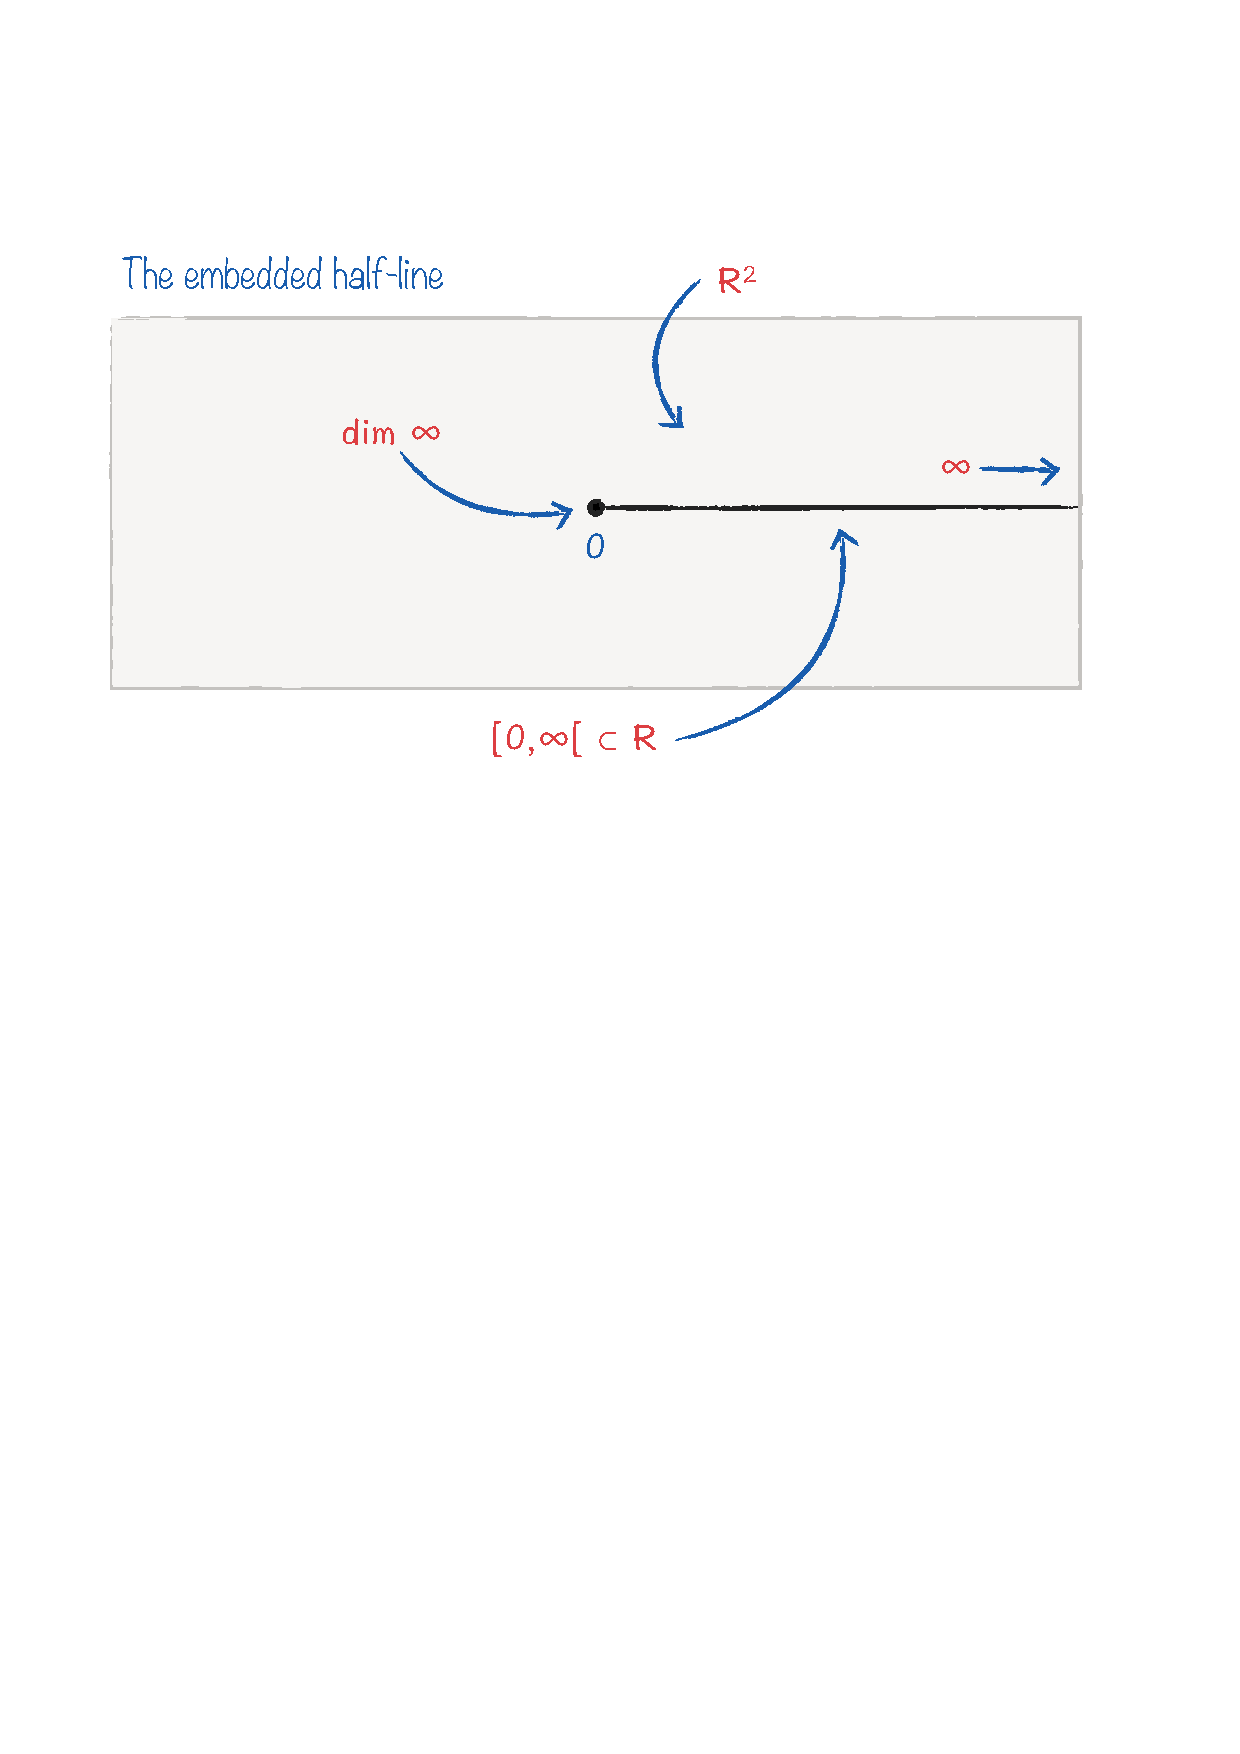
\includegraphics[width=\textwidth]{Figures/embedded-half-line.pdf}}
